\documentclass[11pt,a4paper]{article}
\usepackage[T1]{fontenc}\usepackage[utf8]{inputenc}\usepackage[scaled=0.95]{helvet}\renewcommand{\familydefault}{\sfdefault}
\usepackage[a4paper,margin=2.2cm]{geometry}\usepackage{graphicx,booktabs,caption}\usepackage[hidelinks]{hyperref}\captionsetup{font=small,labelfont=bf}
\setlength{\parindent}{0pt}\setlength{\parskip}{0.6em}
\begin{document}
{\LARGE\textbf{The congregations on rue de Terrebonne in the CRA\textquoteright{}s charity returns, 2015--2024}}\\[3pt]
{\large Is there a pattern across the street\textquoteright{}s places of worship after the 2024 lane?}\\[4pt]
{\small Terrebonne-open-sources, 2026-11-07. Author: a resident of Côte-des-Neiges--Notre-Dame-de-Grâce (see the repository\textquoteright{}s « About the author »). Data: Canada Revenue Agency, T3010 returns as published in the « List of charities » open-data files (open.canada.ca), identification file 2024 and financial files 2015--2024; no information on directors, trustees or officials is read or kept. Code and tables: \url{https://github.com/OpenMobilityData/Terrebonne-open-sources/tree/main/2026-terrebonne-congregations-cra-t3010}.}

\section*{Abstract}
The St Monica folder asked whether the parish\textquoteright{}s returns show the financial hardship attributed to the 2024 lane and found nothing in 2024 standing apart from 2019--2023. This note asks whether the same test can be run on the other places of worship on the street, so that a pattern, or its absence, rests on more than one congregation. The CRA\textquoteright{}s 2024 identification file lists three registered charities in the religious categories with an address on rue de Terrebonne along the lane: the parish of Sainte-Monique (6405), the Yuen Kwok Buddhist Temple (6870, the only other building with a frontage and a drop-off zone, on the south side west of Cavendish) and the Deliverance Church of God 7th Day, whose address is a unit in the residential building at 6350. No United congregation files at a Terrebonne address: the building EXP\textquoteright{}s 2023 study calls « Église Rosedale » has no return of its own in 2024. The temple\textquoteright{}s returns begin with fiscal 2022, so it offers two pre-lane years and one lane year; its 2024 revenue (\$180\,k) and gifts are +7\,\% against 2022--2023 and its expenditures +23\,\%, with the caveat that its 2022 and 2023 figures are identical to the dollar. The parish\textquoteright{}s 2024 revenue (\$251\,k) and gifts (\$220\,k) lie within their 2019--2023 range (+3\,\% and -3\,\% against the five-year mean). The third charity\textquoteright{}s returns are under \$12\,k a year and nil in 2024. On the street itself, then, the pattern test has one comparable congregation besides the parish, with three years of data, and neither shows a 2024 apart from its own earlier years. The 2025 returns, published by the CRA in 2026, will add the first full lane year for both.

\section*{Question}
A financial effect of the lane on a place of worship would come through parking: fewer visitors, lower collections, lower rentals. If it exists, it should appear at every congregation on the same frontage in the same year, and not elsewhere. The St Monica note compared the parish with twelve other Catholic fabriques of the area; this note looks along the street.

\section*{Data}
The 2024 identification file was searched for every registered charity in the religious categories (CRA category codes 0030, 0040, 0050, 0060, 0070) with a Montréal address in the H4A, H4B, H4V and H3X postal areas, and each address was placed on the City\textquoteright{}s assessment roll. Three have an address on rue de Terrebonne between the lane\textquoteright{}s west end and Girouard (Table~\ref{tab:set}). Four more have buildings within the Somerled--Monkland band (First Church of Christ Scientist and Madison Baptist Church on Monkland, St Thomas\textquoteright{} Church on Somerled, St John\textquoteright{}s Lutheran Church on Marcil); they are listed in \texttt{congregations\_band\_candidates.csv} for a later extension and are not used here, the question being the street itself. The financial rows (Section D and Schedule 6 of the T3010) were extracted from the yearly files 2015--2024 for the three business numbers, with the full files\textquoteright{} sizes and SHA-256 recorded in \texttt{raw/open-canada/SOURCES.tsv}. The temple\textquoteright{}s number carries the suffix RR0002; the RR0001 suffix appears in no year, so its series begins with fiscal 2022.
\begin{table}[htbp]\centering\small\caption{Registered charities with a Terrebonne address along the lane (CRA identification file 2024; position from the City roll).}\label{tab:set}
\begin{tabular}{@{}p{3.6cm}p{3.2cm}p{1.6cm}p{7.2cm}@{}}\toprule charity & address & fiscal year end & note\\ \midrule
Sainte-Monique (St Monica) & 6405 rue de Terrebonne & Dec 31 & north side, Benny--Madison, east of Cavendish; church lot and drop-off zone\\
Yuen Kwok Buddhist Temple & 6870 rue de Terrebonne & Dec 31 & south side, Mariette--Rosedale, west of Cavendish; drop-off zone (EXP 2023 p.~40); returns from fiscal 2022\\
Deliverance Church of God 7th Day & 203-6350 rue de Terrebonne & Sept 30 & a unit in a residential building (127 dwellings); no frontage or lot of its own\\
\bottomrule\end{tabular}\end{table}

\section*{Method}
For each congregation, total revenue (line 4700), gifts (4500 receipted plus 4530 not receipted) and total expenditures (5100) by fiscal year; the first fiscal year with the lane in place is the one ending in 2024 (the lane was built in May--June 2024: seven months of it for a December year end, four for a September one). Each 2024 figure is set against the congregation\textquoteright{}s own pre-lane years, 2019--2023 for the two long series and 2022--2023 for the temple: the mean, the range, and whether 2024 falls inside it. No statistical test is attempted on one or three years; the question is whether 2024 stands apart from the congregation\textquoteright{}s own record.

\section*{Results}
\begin{table}[htbp]\centering\small\caption{2024 against each congregation\textquoteright{}s pre-lane years (thousands of dollars).}\label{tab:res}
\resizebox{\textwidth}{!}{\begin{tabular}{@{}llllllrrl@{}}\toprule congregation & line & base years (n) & base mean & base range & 2024 & vs mean & vs 2023 & 2024 in range\\ \midrule
Sainte-Monique (St Monica) & revenue & 2019--2023 (5) & \$244\,k & \$203\,k--\$277\,k & \$251\,k & +3\,\% & -6\,\% & yes \\
Sainte-Monique (St Monica) & gifts & 2019--2023 (5) & \$226\,k & \$195\,k--\$264\,k & \$220\,k & -3\,\% & -6\,\% & yes \\
Sainte-Monique (St Monica) & expenditures & 2019--2023 (5) & \$249\,k & \$198\,k--\$292\,k & \$269\,k & +8\,\% & -2\,\% & yes \\
Yuen Kwok Buddhist Temple & revenue & 2022--2023 (2) & \$168\,k & \$168\,k--\$168\,k & \$180\,k & +7\,\% & +7\,\% & no \\
Yuen Kwok Buddhist Temple & gifts & 2022--2023 (2) & \$168\,k & \$168\,k--\$168\,k & \$180\,k & +7\,\% & +7\,\% & no \\
Yuen Kwok Buddhist Temple & expenditures & 2022--2023 (2) & \$145\,k & \$145\,k--\$145\,k & \$178\,k & +23\,\% & +23\,\% & no \\
\bottomrule\end{tabular}}\end{table}
\begin{figure}[htbp]\centering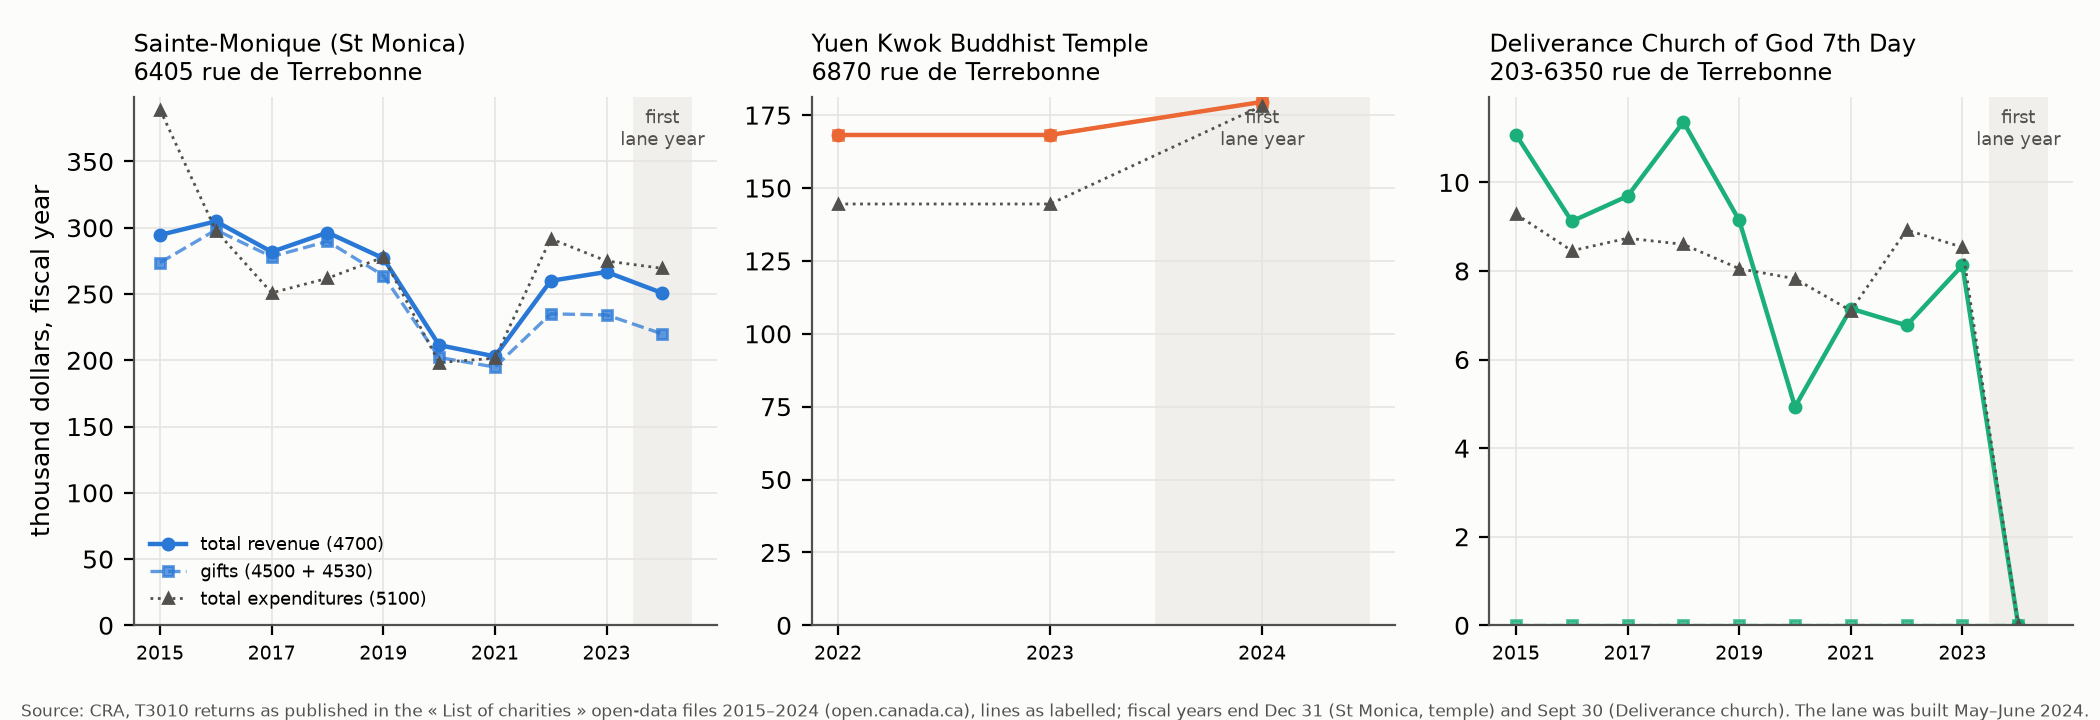
\includegraphics[width=\textwidth]{figures/terrebonne_congregations_series_en.png}\caption{Total revenue, gifts and total expenditures by fiscal year; shaded: the first fiscal year with the lane.}\end{figure}

\textbf{Sainte-Monique.} Revenue 2015: \$295\,k, 2016: \$305\,k, 2017: \$282\,k, 2018: \$296\,k, 2019: \$277\,k, 2020: \$211\,k, 2021: \$203\,k, 2022: \$260\,k, 2023: \$267\,k, 2024: \$251\,k. Gifts 2015: \$274\,k, 2016: \$298\,k, 2017: \$278\,k, 2018: \$290\,k, 2019: \$264\,k, 2020: \$202\,k, 2021: \$195\,k, 2022: \$235\,k, 2023: \$234\,k, 2024: \$220\,k. The 2024 figures fall inside the 2019--2023 range, +3\,\% (revenue) and -3\,\% (gifts) against the five-year mean, -6\,\% and -6\,\% against 2023. The St Monica folder places the 2023$\to$2024 change among the twelve fabriques (median change in gifts +1\,\% there, range -50 to +73\,\%), and its 2025 return, read from the Charities Listings, is the highest revenue since 2016.

\textbf{Yuen Kwok Buddhist Temple.} Revenue 2022: \$168\,k, 2023: \$168\,k, 2024: \$180\,k; all of it reported as gifts; expenditures 2022: \$145\,k, 2023: \$145\,k, 2024: \$178\,k. The 2022 and 2023 returns carry identical revenue and expenditure figures to the dollar, which suggests one year\textquoteright{}s figures were carried into the other; the two-year base is therefore one observation. In 2024 revenue is +7\,\% and expenditures +23\,\% against that base: the first lane year is the temple\textquoteright{}s highest on both lines in its short series.

\textbf{Deliverance Church of God 7th Day.} Revenue of \$5\,k to \$11\,k a year from 2015 to 2023 (fiscal years ending September 30), no gifts reported on lines 4500 or 4530, and a 2024 return with every financial line at zero: a nil or incomplete return, uninformative for this question, and in any case a congregation without a frontage on the street.

\section*{Discussion}
On the street itself the pattern test is thin by construction: one parish with a decade of returns, one temple with three years of which two are identical, and one congregation that meets in a residential unit. What the data allow is a negative statement at both buildings with a frontage: neither congregation\textquoteright{}s first lane year stands apart from its own earlier years, and at both the 2024 figures are at or above the pre-lane mean. Nothing in the returns distinguishes the side converted in winter (the temple\textquoteright{}s block converts its north side, the church\textquoteright{}s block its south side; the temple faces the converted side across the street, the church does not). The limits are those of the St Monica note: annual totals, no monthly series, gifts that move with membership and events, and the CRA\textquoteright{}s publication lag. The 2025 returns of the two congregations, in the 2025 open-data file expected in 2026, will give the first full calendar year with the lane for both; the four congregations within a block, already identified, would extend the test to the band if wanted.

\section*{Reproducibility}
\texttt{fetch\_congregations.py} downloads the yearly financial file and keeps the rows of the business numbers in \texttt{congregations.csv}; \texttt{congregations\_comparison.py} writes \texttt{congregations\_long.csv}, \texttt{summary.json} and the figure; \texttt{build\_note.py} writes this note. Generated 2026-11-07 12:47.
\end{document}
